\section{دسته‌بندی رابطه با بهره‌گیری از مدل \lr{BERT} و کانولوشن‌های تکه‌ای به همراه خطای کسری \cite{bert}}

در سال ۲۰۲۱ لیو\LTRfootnote{Liu} و همکارانش رویکرد متفاوتی را در رابطه با شبکه‌های عصبی پیچشی تکه‌ای در پیش گرفتند.
آن‌ها به جای این که یک کانولوشن را روی شبکه انجام داده و خروجی آن‌ را سه قسمت کنند سه کانولوشن متفاوت را
روی سه قسمت جمله اجرا کردند. با ترکیب خروجی‌های این سه قسمت رابطه‌ای که جمله بیان می‌کند تشخیص داده می‌شود.

\begin{figure}[h]
    \centering
    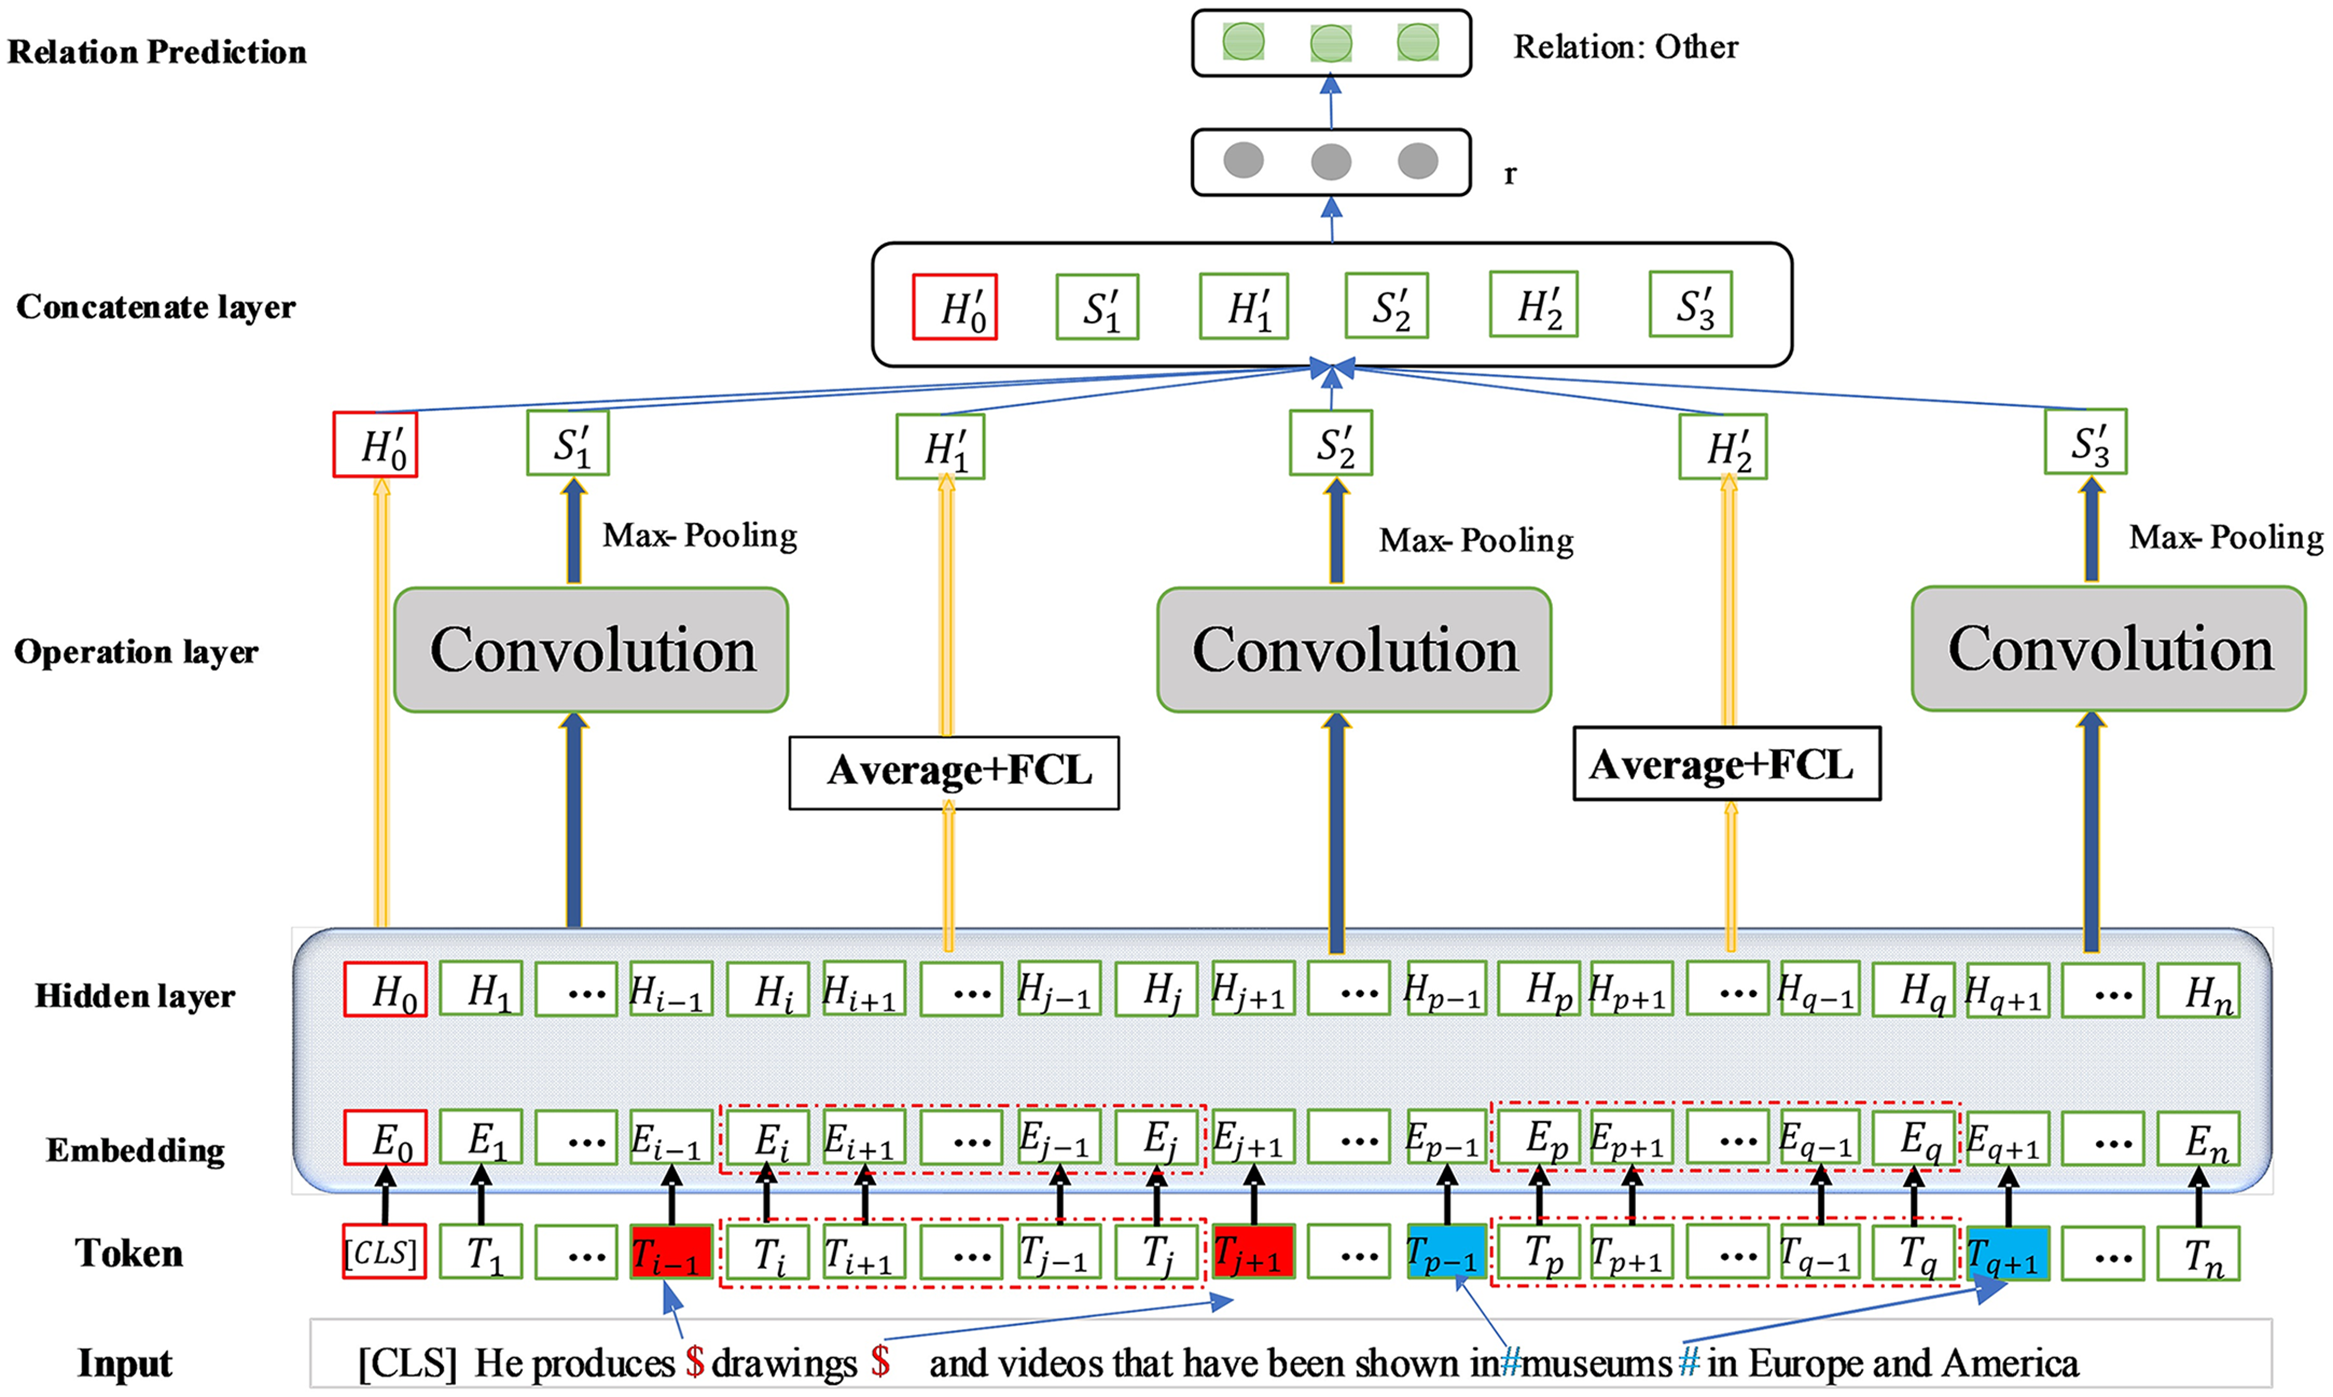
\includegraphics[width=\linewidth]{images/bert/architecture.png}
    \caption{ساختار مدل پیشنهادی}
    \label{article1_architecture}
\end{figure}

مدل پیشنهادی لیو و همکارانش در شکل \ref{article1_architecture} دیده می‌شود. مدل پیشنهادی آن‌ها انتظار دارد موجودیت‌های موجود
در جمله با علامت مخصوصی نظیر $\$$ و $\#$ مشخص شده باشد. با دریافت جمله، توکن‌های \lr{[CLS]} و
\lr{[SEP]} به جمله اضافه شده و جمله به مدل \lr{BERT} داده می‌شود. پس از دریافت بازنمایی کلمات $(E_i)$ از مدل \lr{BERT} هر
بازنمایی از یک لایه \lr{Dense} عبور کرده و بازنمایی دیگری به نام $H_i$ را تولید می‌کند. در این مرحله بازنمایی توکن‌ها
به شش دسته تقسیم شده و برای هر بخش روند متفاوتی طی می‌شود.

\begin{itemize}
    \item \textbf{توکن آغاز جمله \lr{BERT}}: بر روی بازنمایی این توکن عملیات خاصی انجام نشده و مستقیما به خروجی
    منتقل می‌شود.
    \item \textbf{کلمات قبل از موجودیت اول}: بازنمایی متناظر این کلمات $(H_i)$ ها از یک لایه کانولوشن عبور کرده و
    در قدم بعدی \lr{max pooling} گرفته می‌شود. به عبارت ریاضی
    \begin{flalign}
        X_{i:i+h-1} & = H_i \oplus H_{i+1} \oplus H_{i+2} \oplus ... \oplus H_{i+h_1} \\
        c_i & = W * X_{i:i+h-1} + b
    \end{flalign}
    در عبارت بالا منظور از عملگر $\oplus$ عملگر \lr{concatenation} منظور از عملگر $*$ کانولوشن است.
    بنابراین $c_i$ یک عدد بردار در فضای $\mathbb{R}^d$ است. با اعمال این کانولوشن با پنجره $h$
    روی بازنمایی کلمات ماتریس $C$ به شکل زیر تولید می‌شود. ماتریس $C$ در فضای $\mathbb{R}^{(n-h+1) \times d}$
    است.
    \begin{flalign}
        C = \left[ c_1, c_2, ..., c_{n-h+1}\right]
    \end{flalign}
    حال بر روی این ماتریس عملیات \lr{max pooling} انجام می‌شود. هدف از انجام این عملیات علاوه بر کاهش
    ابعاد به فضای $\mathbb{R}^{n-h+1}$، انتخاب مهم‌ترین ویژگی از هر یک از $c_i$هاست.
    \begin{flalign}
        s = \max(C)
    \end{flalign}
    بردار $s$ به مرحله بعدی منتقل می‌شود.
    \item \textbf{موجودیت اول}: از آن جا که ممکن است موجودیت اول خود شامل چند کلمه و در نتیجه دارای بازنمایی چندبعدی باشد بنابراین
    ابتدا میانگین این بازنمایی را پیدا کرده و به عنوان بازنمایی موجودیت اول در نظر می‌گیریم. با عبور این بازنمایی از
    یک لایه \lr{Dense} مقدار $H'_1$ تولید می‌شود. به عبارت ریاضی
    \begin{eqnarray}
        H'_1 = W_1(\tanh(\frac{1}{j-i+1} \sum_{t=i}^{j}{H_t})) + b_1
    \end{eqnarray}
    \item \textbf{کلمات بین دو موجودیت}: برای این کلمات علمیات مشابهی مانند عملیات انجام شده بر روی کلمات
    قبل از موجودیت اول انجام می‌شود.
    \item \textbf{موجودیت دوم}: در این حالت نیز عملیات مشابهی نظیر عملیات انجام شده روی موجودیت اول انجام می‌شود.
    \item \textbf{کلمات بعد از موجودیت دوم}: عملیات انجام شده در این قسمت مشابه عملیات انجام شده روی کلمات
    قبل از موجودیت اول است.
\end{itemize}

پس از استخراج بردار‌های متناظر هر قسمت یعنی $H'_0$، $H'_1$، $H'_2$، $S'_1$، $S'_2$ و $S'_3$ این بردار‌ها با هم
ترکیب شده و به یک لایه \lr{Dense} با تابع فعال‌سازی \lr{softmax} داده می‌شوند.
بیان ریاضی این عملیات به شرح زیر است.

\begin{flalign}
    r = & \; W_r(H'_0 \oplus S'_1 \oplus H'_1 \oplus S'_2 \oplus H'_2 \oplus S'_3) + b_r \\
    \tilde{y} = & \; \sigma(r)
\end{flalign}

در روابط بالا منظور از $\sigma$ تابع \lr{softmax} است. این تابع برای هر دسته یک احتمال نسبت می‌دهد. دسته‌ای که بیشترین
احتمال را داشته باشد به عنوان خروجی نهایی مدل در نظر گرفته می‌شود.

\subsection{تابع خطا}

بیشتر پژوهش‌هایی که در زمینه استخراج رابطه انجام شده‌اند از تابع خطای آنتروپی متقابل\LTRfootnote{cross entropy} که به شرح زیر
تعریف می‌شود برای محاسبه خطای مدل استفاده کرده‌اند. مشکلی که این تابع دارد این است که نسبت به
کلاس‌های با تعداد نمونه زیاد (و در نتیجه آسان بودن یادگیری این کلاس‌ها) بایاس داشته و اعداد
بالایی را برای آن‌ها گزارش می‌دهد.

\begin{flalign}
    J(\theta) = - \sum_{i} y_i \log(p_t) + (1-y_i) \log(1-p_t)
\end{flalign}

برای رفع مشکل این مشکل لیو و همکاران از ایده‌ای که در سال ۲۰۱۷ توسط لین و همکارانش \cite{focal-loss} ارائه شد،
استفاده کرده‌اند. تابع خطای معرفی شده توسط لین تابع خطای کسری\LTRfootnote{focal loss} نامیده شده و به شرح زیر
تعریف می‌شود.

\begin{flalign}
    FL(p_t) = - a_t (1-p_t)^{\gamma} \log(p_t)
\end{flalign}

در این فرمول $\alpha_t$ فاکتور وزن‌دهی نامیده شده و مقداری بین $\left[0,1\right]$ دارد. $\gamma$ نیز پارامتر توجه
نامیده می‌شود. $p_t$ نیز احتمالی است که مدل با آن احتمال درصد اطمینان را گزارش می‌دهد.
برای روشن‌تر شدن مفهوم هر یک از این پارامتر‌ها از یک مثال استفاده می‌کنیم.

فرض کنید دو دسته داریم که فراوانی هر یک از تعداد کل داده‌ها به ترتیب $0.1$ و $0.25$ باشد. همچنین فرض کنید دو مدل
مختلف نیز داریم. مدل اول روی دسته با فراوانی کم‌تر با اطمینان $0.8$ و روی دسته با فراوانی بیشتر با اطمینان $0.85$ درصد
پیش‌بینی انجام می‌دهد. مدل دوم در دسته با فراوانی کم‌تر با اطمینان $0.6$ و در دسته با فراوانی زیاد با اطمینان $0.95$ درصد
پیش‌بینی انجام می‌کند. اگر بخواهیم این عملکرد این دو مدل را با تابع خطای \lr{cross entropy} نسبت به هم بسنجیم،
خواهیم داشت.

\begin{flalign}
    FL(\text{\lr{model}}_1) = & - 0.1 \times (1-0.8)^2 \times \log(0.8) - 0.25 \times (1-0.85)^2 \times \log(0.85) \simeq 0.002 \\
    FL(\text{\lr{model}}_2) = & - 0.1 \times (1-0.6)^2 \times \log(0.6) - 0.25 \times (1-0.95)^2 \times \log(0.95) \simeq 0.008
\end{flalign}

همان‌طور که مشاهده می‌شود تابع خطای کسری برای مدل دوم عدد بزرگتری را گزارش می‌دهد که منطقی است. چرا که مدل دوم در زمانی
که داده بیشتری داشته بهتر و زمانی که با کمبود داده مواجه بوده است عملکرد ضعیفی داشته است. در این مثال مقدار $\gamma=2$
و مقدار $\alpha_t$ را نسبت داده‌های دسته به تعداد کل داده‌ها در نظر گرفتیم. در این مقاله نیز مقدار $\alpha_t$ به همین شکل
انتخاب می‌شود.

حال که با چگونگی رفتار تابع خطا آشنا شدیم، چگونگی اعمال این ایده در تابع آنتروپی متقابل را
مطالعه می‌کنیم. با اعمال این ایده تابع خطای آنتروپی متقابل به شکل زیر در می‌آید.

\begin{flalign}
    J(\theta) = - \sum_{i} \alpha_t y_i (1-p_t)^{\gamma} \log(p_t) + \alpha_t (1-y_i) p_t^{\gamma}\log(1-p_t)
\end{flalign}

این تابع خطا به خوبی دسته‌های با برچسب کم را در نظر می‌گیرد. در این مقاله علاوه بر این کار یک مقدار منظم‌سازی نیز روی
تابع اعمال شده و تابع خطا به شکل زیر حاصل می‌شود.

\begin{flalign}
    J(\theta) = - \sum_{i} \alpha_t y_i (1-p_t)^{\gamma} \log(p_t) + \alpha_t (1-y_i) p_t^{\gamma}\log(1-p_t) + w ||\theta||^2
\end{flalign}

وزن‌های مدل با استفاده از این تابع خطا به روز می‌شود.
